\section{Biological Productivity}\label{sec:npp}

\subsection{Revisiting the Impact of Mesoscale Eddies}\label{sec:npp-mechanisms}

\Textcite{mcgilli-2016-meso-review} identified two important mesoscale processes that impact the productivity in an \ac{ebus}: lateral export of biomass by eddy stirring (described by \textcite{rossi-2008-stirring} for Canary \ac{ebus}) and the subduction of upwelled nutrients (also called eddy quenching, described by \textcite{gruber-2011-eddy-red} for California \ac{ebus}). Both processes are briefly discussed with data from \ac{mr}.\\
\\
Eddy composites of surface chlorophyll anomalies indicate that mesoscale eddies trap water masses and stir surrounding water. The composites are shown in \autoref{fig:chl-anomaly} and are very similar to observations from \textcite[see their Figure 9d]{gaube-2014-observations-mesoeddies}. A decomposition reveals a strong monopole contribution and a dipole-like residual. The monopole can be a result of eddy pumping or trapping \autocite{gaube-2014-observations-mesoeddies}. Because the \ac{cc} flows southward and upwelling of nutrients is strongest close to the coast, cyclones trap in general nutrient rich water whereas anticyclones trap nutrient depleted water \autocite{nagai-2015-dom-role-meso}. This matches the sign of the observed monopole contribution in the surface chlorophyll anomaly. Hence, the occurrence of trapping can be verified. But in contrast to \textcite{gaube-2014-observations-mesoeddies}, there is no indication for eddy pumping which would appear as an intensification of the anomaly during the first days of an eddy track. However, this finding strongly relies on the tracking algorithm (see \autoref{sec:mesoscale-comparison}) and the authors note that the trend is not significant in their results either. The fact that stirring takes place can be seen in the dipole structure of the residual. The structure reflects the theoretical imprint of a westward travelling vortex in a tracer field with an east-to-west gradient \autocite[see their Figure 3]{chelton-2011-surfacechl}. In the case of the \ac{ccs}, this gradient is produced by coastal upwelling.\\
\begin{figure}
    \centering
    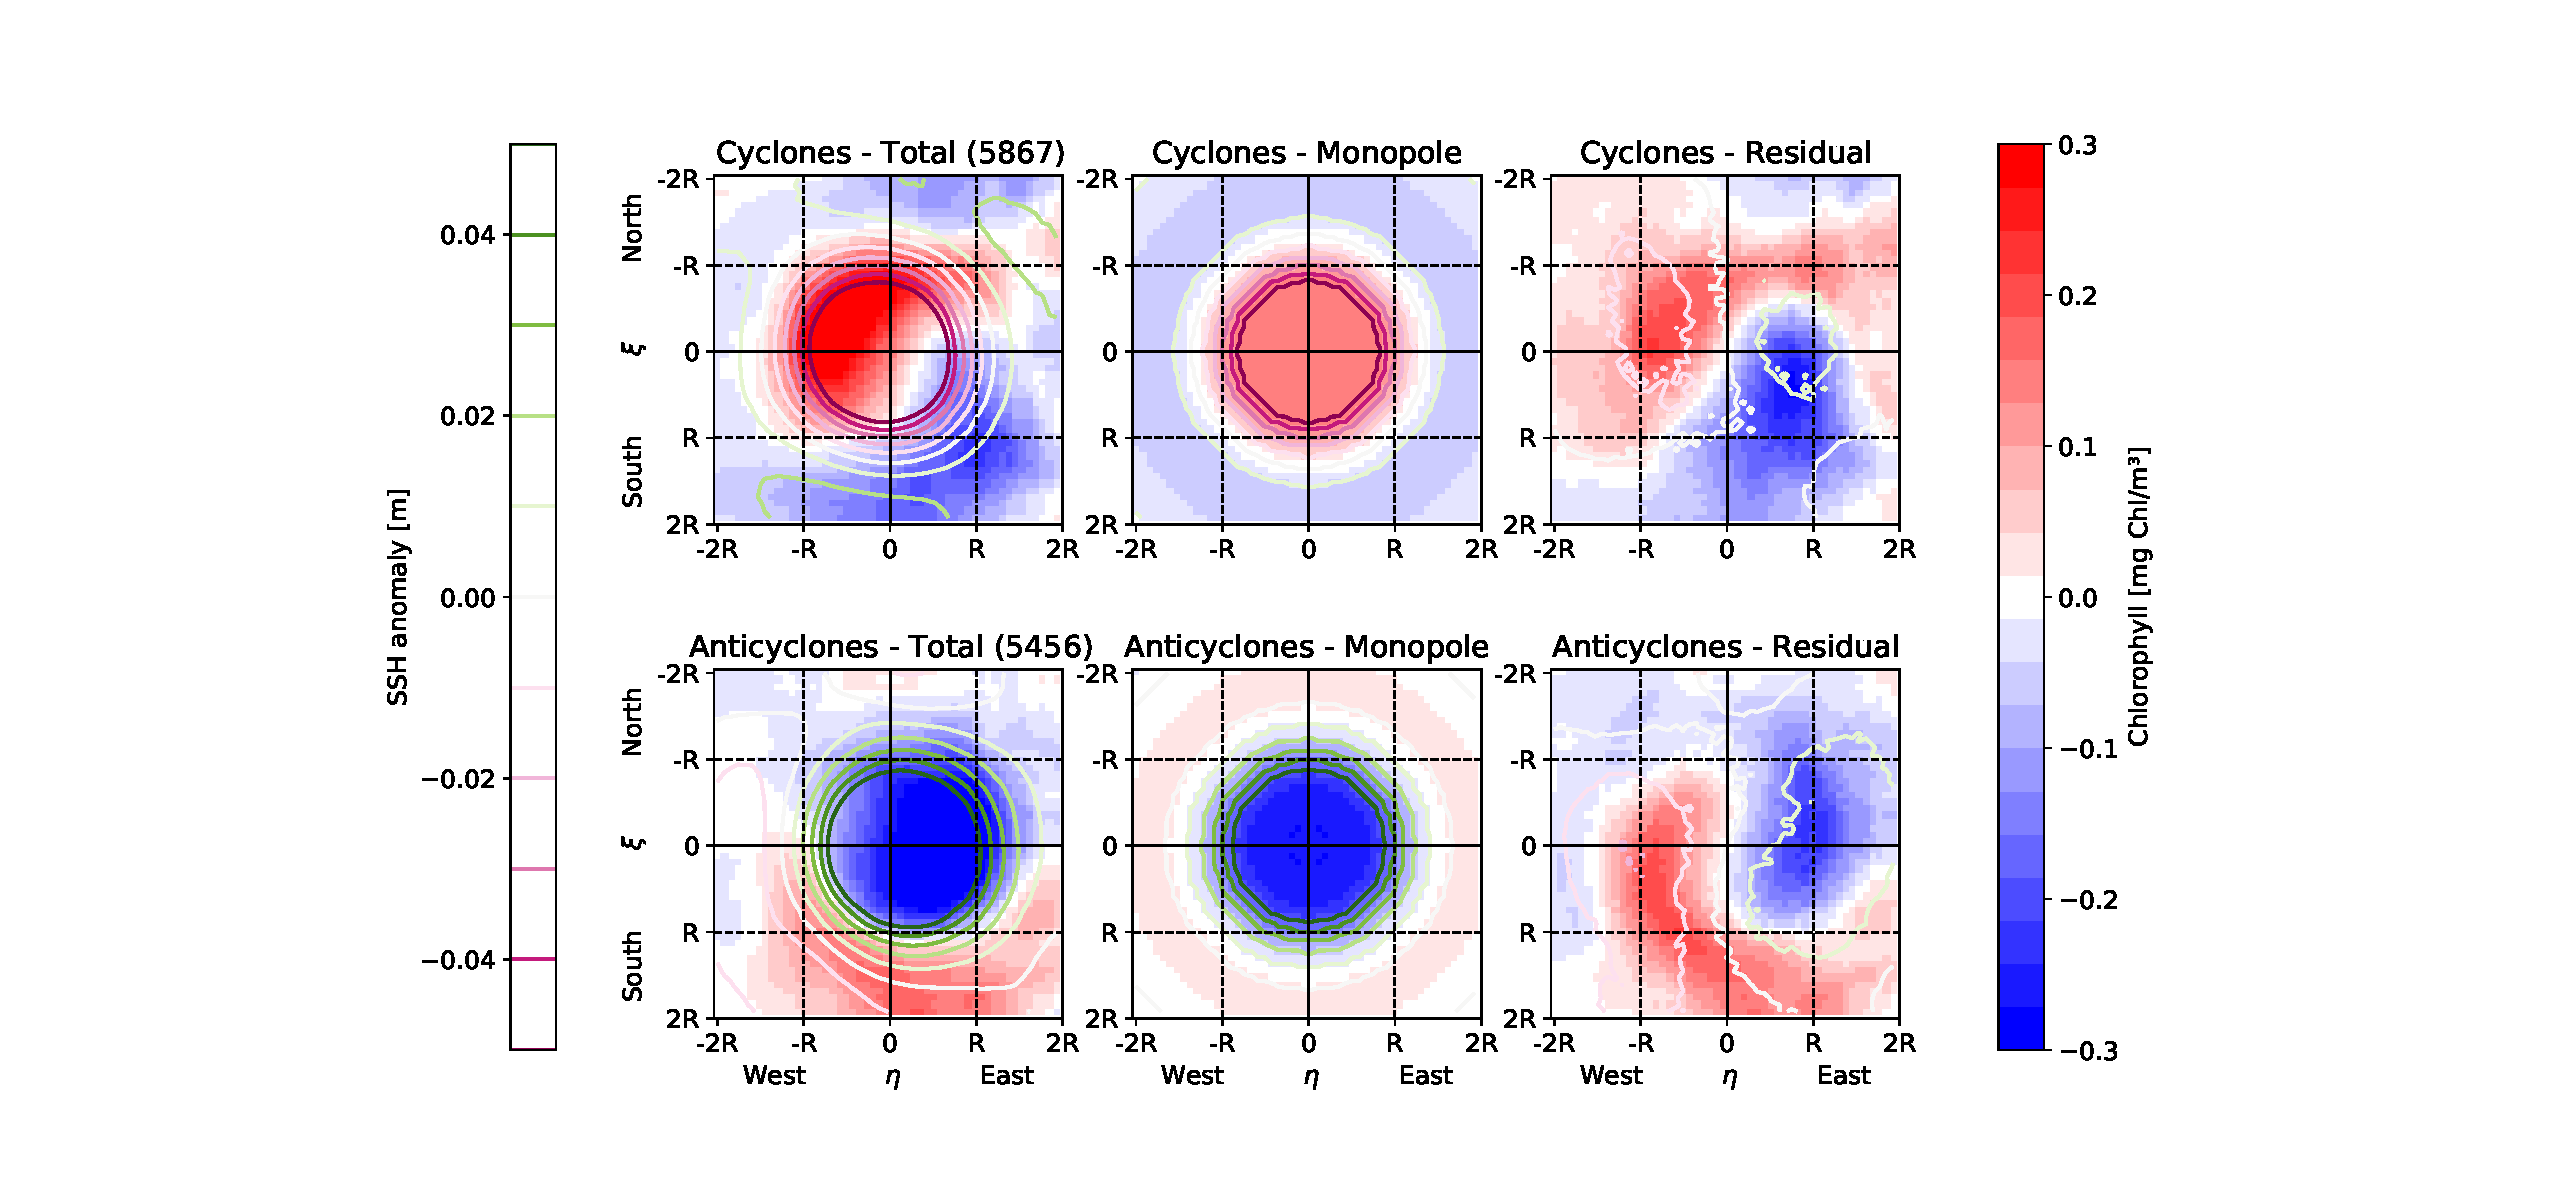
\includegraphics[width=18cm, trim=6.5cm 0 0 0]{../figures/result_composites_chl.pdf}
    \caption[Average surface CHL anomaly]{\textbf{Average surface CHL anomaly.} The total averaged CHL anomaly (left) was decomposed into a monopole by a radial mean (center) and a residual (right). The top row corresponds to cyclones, the bottom row to anticyclones. The contours represent SSH anomalies. The number of aggregated eddies is denoted in brackets.}\label{fig:chl-anomaly}
\end{figure}
\\
Mesoscale eddies induce to a subduction of nutrients to an intermediate layer ($\around \SI{100}{\metre}$) at which the nutrients are exported offshore. This effectively removes nutrients from the upwelling cycle and leads to a reduction of productivity at the coast in the long run \autocite{gruber-2011-eddy-red}. \Textcite{gruber-2011-eddy-red} visualize the process using the eddy-induced nitrate flux $\mathbf{j}_e$ which is given as
\begin{align}
\mathbf{j}_e = \text{TN}'\textbf{u}' = (\text{TN} - \overline{\text{TN}})(\textbf{u} - \overline{\textbf{u}})
\end{align}
where TN is the total nitrogen and $\mathbf{u}$ the velocity. The vertical and horizontal (perpendicular to the coastline) component of $\mathbf{j}_e$ are shown in \autoref{fig:gruber-n-flux}. The components compare very well to the flux observed by \textcite[see their Figure 4]{gruber-2011-eddy-red}, both in magnitude and location of up- and downwelling zones. The flux observed in this study omits a horizontal transport close to the surface and the upwelling region at the coast is slightly tighter. However, these differences do not impact the mechanism itself.
\begin{figure}
        \centering
        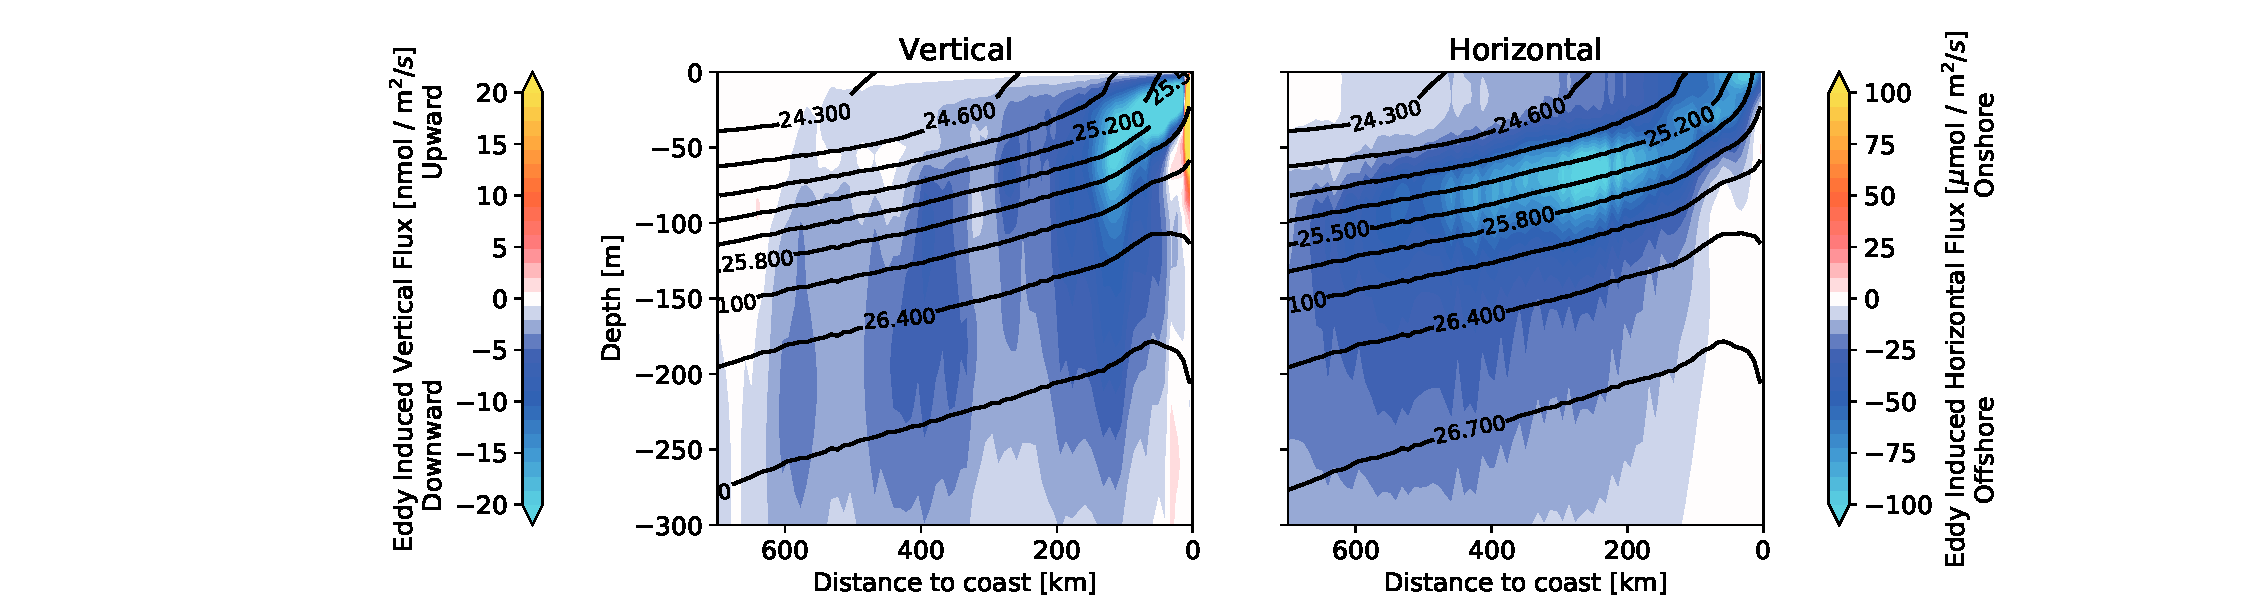
\includegraphics[width=17cm, trim=6.5cm 0 0 0]{../figures/result_eddy_quenching.pdf}
        \caption[Eddy-induced total nitrate flux]{\textbf{Eddy-induced total nitrate flux.} The vertical component is shown left and the horizontal component right. Black lines denote isopycnals. Note the different order of magnitude and different color scale for the two components.}\label{fig:gruber-n-flux}
\end{figure}

\subsection{NPP in MR and HR}\label{sec:npp-dist}

Biological productivity is highest at the coast and decreases continuously with distance to coast in both models (see \autoref{fig:npp_domain}). The reason for this is that Ekman induced upwelling of nutrients fuels productivity at the coast from where nutrients and organic matter are transported offshore by mesoscale processes \autocite{nagai-2015-dom-role-meso}. Compared to satellite observations (see \autoref{fig:npp_domain}) and comparable numerical models (e.g. \textcite[see their Figure 5]{deutsch-2020-subm-modeldescr}) both, \ac{mr} and \ac{hr}, overestimate \ac{npp} at the coast. This is probably related to a bad tuning of the model parameters to the new atmospheric forcing (see \autoref{sec:data-methods-model}, internal communication). However, conclusions are mainly drawn from the difference between \ac{mr} and \ac{hr} which should be less affected than the absolute values.\\
\begin{figure}
    \centering
    \hspace*{0.2cm}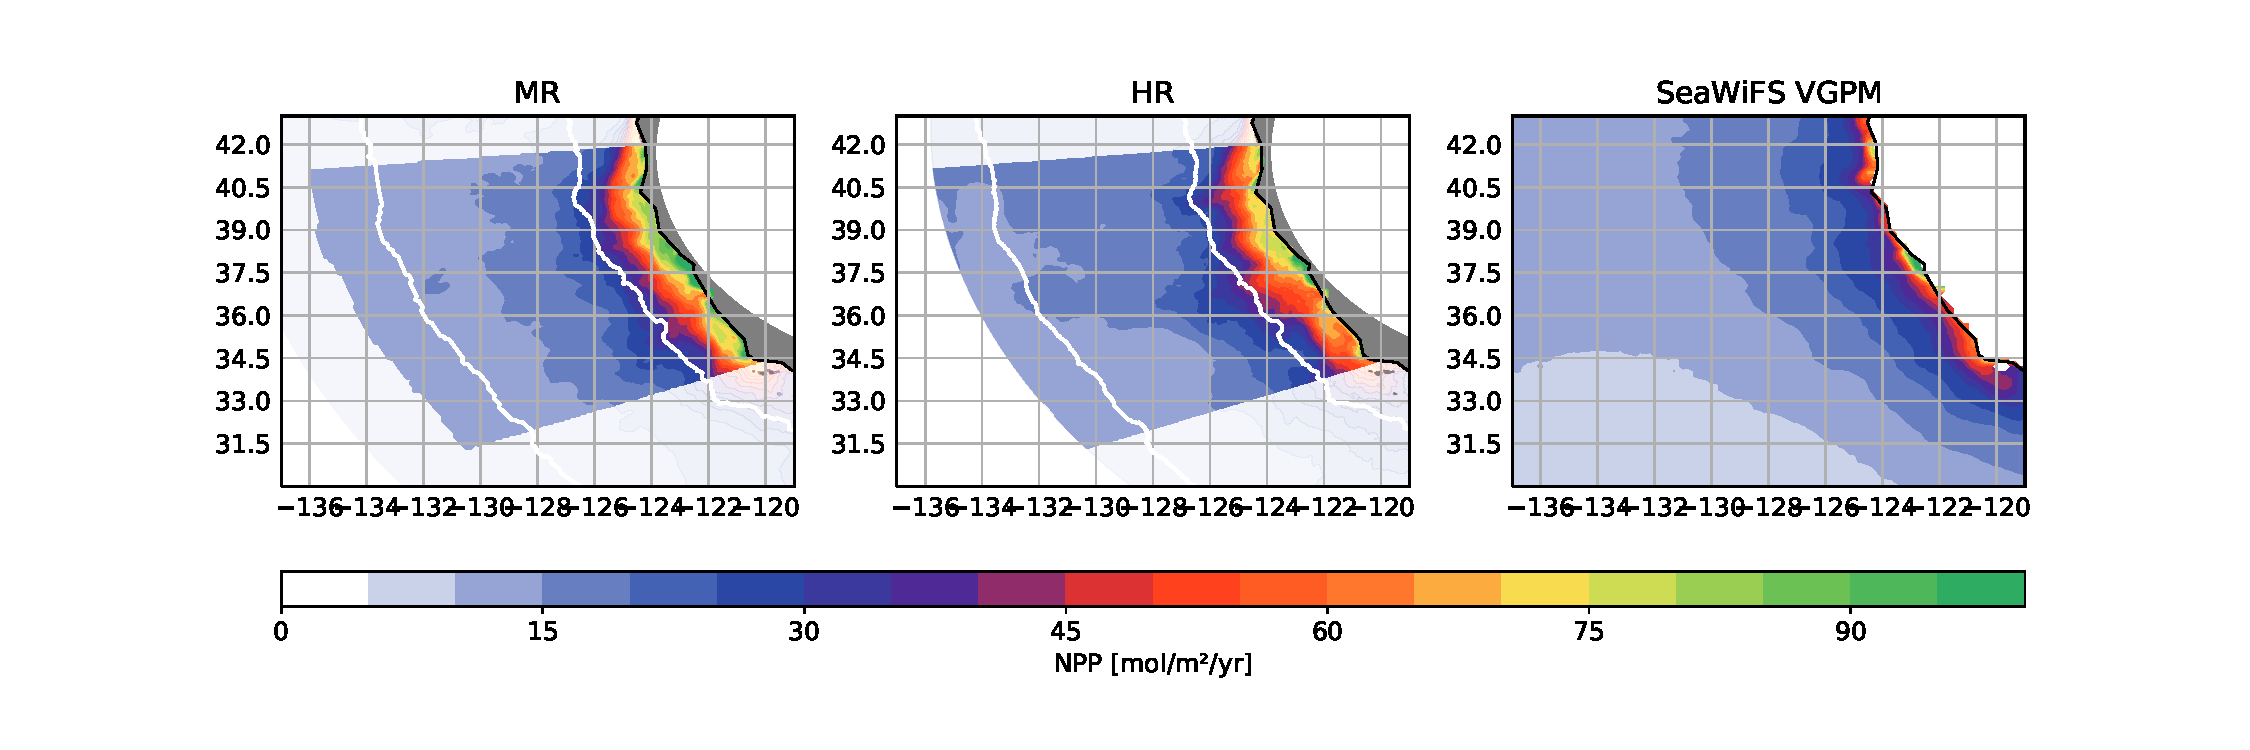
\includegraphics[width=16cm, trim=3cm 0 0 0]{../figures/result_npp_domain.pdf}
    \caption[Spatial distribution of NPP]{\textbf{Spatial distribution of NPP} in \ac{mr} (left) and \ac{hr} (center). \ac{npp} was integrated vertically and averaged over integration time. White lines denote $200\si{\kilo\metre}$ and $800\si{\kilo\metre}$ distance to coast. \ac{npp} derived from SeaWiFS data (1998-2007) using VGPM algorithm \autocite{behrenfeld-1997-vgpm} is shown right.}
    \label{fig:npp_domain}
\end{figure}
\\
Compared to \ac{mr}, \ac{npp} is reduced in \ac{hr} by $\SI[separate-uncertainty]{3.8(13)}{\percent}$ in the nearshore region and by $\SI[separate-uncertainty]{11.0(17)}{\percent}$ within $50\si{\kilo\metre}$ off the coast (see \autoref{fig:npp_d2c}). The temporal and spatial distribution of \ac{npp} is shown in \autoref{fig:npp_diff}. The maximum difference between \ac{mr} and \ac{hr} appears in August, but the reduction starts already in April. This is similar to results of \textcite{kessouri-2020-seasonal-prod} who compare two models of the \ac{ccs} with horizontal resolutions of $\SI{4}{\kilo\metre}$ and $\SI{1}{\kilo\metre}$. They also observe a reduction of \ac{npp} in the high-resolution model by up to $\SI{10}{\percent}$ within $\SI{200}{\kilo\metre}$ off the coast and a maximum of the reduction in August. However, the reduction starts about a month later than observed in this study. Possible reasons for this delay are discussed in \autoref{sec:discussion}.\\
\begin{figure}
    \centering
    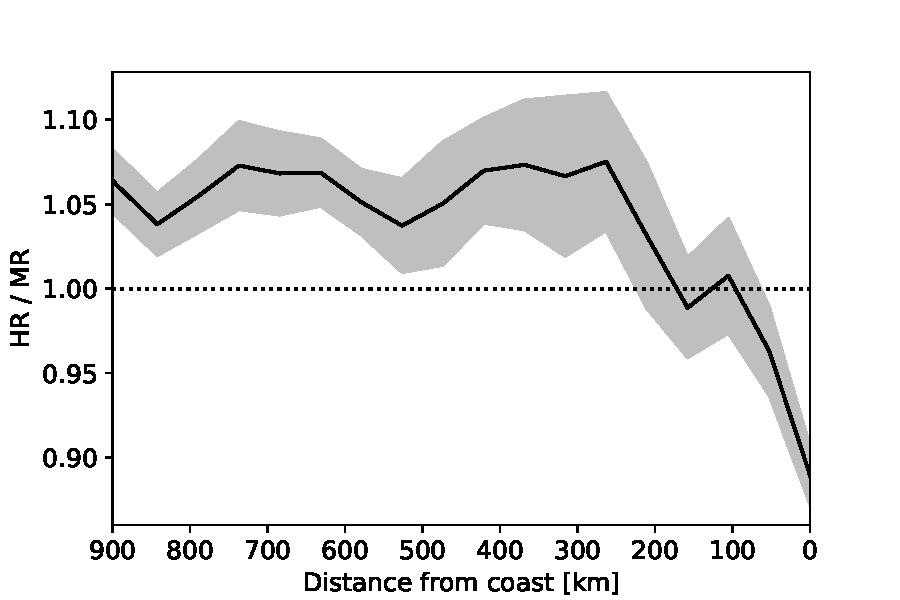
\includegraphics[width=8cm, trim=0 0 0 0]{../figures/result_npp_reduction.pdf}
    \caption[Relative change of NPP with distance from coast]{\textbf{Relative change of NPP with distance from coast}. The shaded region represents the interannual variability.}
    \label{fig:npp_d2c}
\end{figure}
\begin{figure}
    \centering
    \hspace*{0.3cm}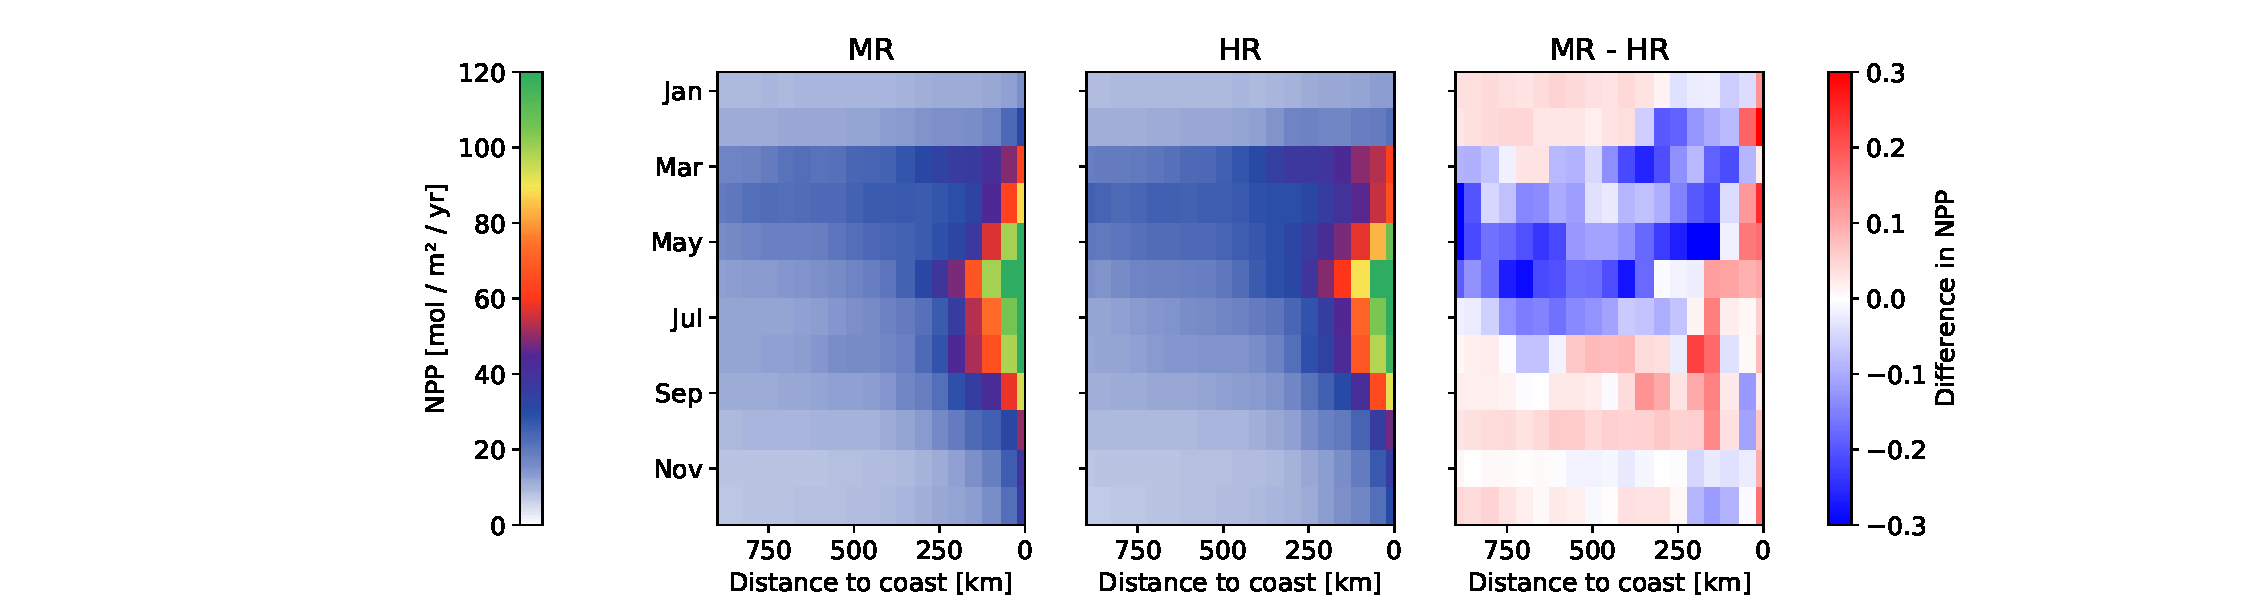
\includegraphics[width=17cm, trim=7cm 0 0 0]{../figures/result_npp_diff.pdf}
    \caption[Hovmöller diagram of NPP]{\textbf{Hovmöller diagram of NPP} for \ac{mr} (left) and \ac{hr} (right). The relative difference (\ac{mr}  - \ac{hr})/\ac{mr} is shown (right).}\label{fig:npp_diff}
\end{figure}
\\
In the offshore region, \ac{npp} is increased in \ac{hr} by $\SI[separate-uncertainty]{6.0(9)}{\percent}$ (see \autoref{fig:npp_d2c}). During spring, when offshore productivity is highest in both models, the difference increases to $\SI[separate-uncertainty]{14.4(20)}{\percent}$. Contrary to this, \textcite{kessouri-2020-seasonal-prod} observe a year-round offshore increase in \ac{npp} with a maximum increase in late spring (see their Figure 6). This discrepancy is discussed in detail in \autoref{sec:discussion}.\\
\\
The observed differences in \ac{npp} between \ac{mr} and \ac{hr} have not converged and are still drifting at the end of integration. This can be seen in \autoref{fig:npp_drift} which shows the difference in \ac{npp} for the nearshore and offshore region as a function of integration time. The increase in offshore \ac{npp} stabilizes after two years. This is the reason why the first two years were excluded from the analyses. However, the reduction of nearshore \ac{npp} strengthens throughout the integration time. Because the reduction is related to transport processes and redistribution of nutrients, this can also impact offshore productivity over time. Hence, it is very likely that the distribution of \ac{npp} in \ac{hr} is not fully captured within the short integration time.